\documentclass[12pt]{article}



% lua
\usepackage{luacode}



% Geometry
\usepackage{geometry}
\geometry{
	a4paper, % 210mm por 297mm
	top=15mm,
	left=15mm,
	right=15mm
}



% Linguagem
\usepackage[portuguese]{babel}	% Babel
%\usepackage{polyglossia}		% Polyglossia
%\setdefaultlanguage[variant=brazilian]{portuguese}



% Graphics
\usepackage{graphics}
\graphicspath{ {../resources/} }



% calc
\usepackage{calc}



% Table of contents
\usepackage{tocloft}
\setcounter{tocdepth}{2}	% remove subsubsection from toc

% part
\renewcommand\cftpartfont{\bfseries}
%\renewcommand\cftpartafterpnum{\vspace{0mm}}
\setlength\cftbeforepartskip{6mm}

% sec
\renewcommand\cftsecfont{\bfseries} % Font
\renewcommand\cftsecpagefont{}	 % page number font
\renewcommand\cftsecleader{\cftdotfill{\cftdotsep}} % Dots
\setlength\cftbeforesecskip{3mm}
\setlength\cftsecindent{0mm}
%\setlength{\cftsecnumwidth}{25mm}		% Fix section width

% subsec
\setlength\cftsubsecindent{0mm}
%\setlength{\cftsubsecnumwidth}{15mm}

% tab (table)
\setlength\cfttabindent{0mm}



% filecontents
%\usepackage{filecontents}	% Create files



% Multicols
\usepackage{multicol}
\setlength{\columnsep}{5mm}



% enumitem
\usepackage{enumitem} % modify enumerate index



% titlesec
\usepackage{titlesec}

% Part customization
\titleclass{\part}{straight}
\titleformat{\part}
	[block]							% shape
	{\huge\bfseries\color{Emph}}			% format
	{\thepart\hspace{5mm}{$|$}}			% label
	{5mm}							% sep
	{\huge\bfseries}					% before-code
	[\vspace{0.5mm}]					% after-code
\counterwithin*{section}{part} % Reset section on part
%\@addtoreset{section}{part}
%
%% Chapter customization
%\titleclass{\chapter}{straight}
%\titleformat{\chapter}
%	[block]
%	{\Huge\bfseries\color{Emph}}
%	{\thechapter\hspace{5mm}{$|$}}
%	{5mm}
%	{\Huge\bfseries}
%	[\vspace{0.5mm}]



% Appendix
\usepackage{appendix}



% siunix: SI units
\usepackage{siunitx}
\sisetup{
	scientific-notation = false,	% scientific / engineering / false
	exponent-to-prefix = true,
	exponent-product = *,
	round-mode = places,		% figures/places
	round-precision = 2,
%	round-minimum = 0.01
}



% Maths
\usepackage{amsmath, amssymb}
\usepackage{bm} % Boldmath

\newcommand{\BM}[1]{{\large\boldmath\bfseries%
	\begin{align*}
		#1
	\end{align*}%
}}
%
%\newcommand\vizinhanca[2][\delta]{%
%	\hyperref[vizinhanca]{V_{#1}(#2)}%
%}
%
%\newcommand\converge{{\,\xrightarrow{\text{converge}}\,}}



%% Vectors
%\usepackage{esvect} 	% Vector over-arrow
%\renewcommand{\vec}{\vv} % Vecto over-arrow



%% Tikz
\usepackage{tikz}		
%\usepackage{pgfmath}  	% calculations
%\usepackage{varwidth}  % List inside TikzPicture


%%% pgf
%% pgfmath
%\usepackage{pgfmath}  	% calculations
%
%% pgfplots
%\usepackage{pgfplots}
%	\pgfplotsset{
%		compat=newest,
%		width=.90\textwidth,	% width
%		height= .22\textheigth,	% height
%		major grid style= {
%			very thin, 
%			color= White!60!Black
%		},
%		ticklabel style={
%			/pgf/number format/.cd,
%				set thousands separator={\,},
%		tick style= {color= White!60!Black},
%		% Extra ticks
%		},
%		every extra x tick/.style={
%			tick style= {draw=none},
%			major grid style= 
%				{draw, thin, color= White!90!Black},
%			ticklabel pos= top,
%		},
%		every extra y tick/.style={
%			tick style= {draw=none},
%			major grid style= 
%				{draw, thin, color= White!90!Black},
%			ticklabel pos= right,
%		},
%	}
%
% pgfplotstable
%\usepackage{pgfplotstable}



% Tabular
\usepackage{multirow}
\usepackage{float}	% table position H(ere)
\restylefloat{table}
\usepackage{longtable}
 
\setlength\tabcolsep{6mm}		% Width
\renewcommand\arraystretch{1.25}	% Height

% booktabs
\usepackage{booktabs}
\setlength\heavyrulewidth{.75pt} 	% Top and bottom rule
\setlength\lightrulewidth{.50pt} 	% Middle rule
\usepackage{colortbl} 			% Color Cells



% Chem
\usepackage{chemformula} 	% formulas quimicas
\usepackage{chemfig} 		% Estruturas quimicas
\usepackage{modiagram}		% Molecular orbital diagram
\setmodiagram{
	names, 
	labels, 
	labels-fs=\tiny, 
	AO-width=6mm,
}

\newcommand{\mol}[1]{ \unit{\mole\of{\ch{ #1 }}} } % mol



% Colors
\usepackage{xcolor}

\definecolor{DarkBlue}  {HTML}{252A36}
\definecolor{LightGreen}{HTML}{7CCC6C}
\definecolor{DarkGreen} {HTML}{008675}

\colorlet{White}{DarkGreen!20}
\colorlet{Black}{DarkBlue!110}
%\colorlet{Black}{DarkBlue!70!black}
\colorlet{Emph}{ DarkGreen!70!White}
\colorlet{EmphLight}{Emph!60!White}
\colorlet{Background}{White!5!Black}

\pagecolor{Black}
\color{White}

% mycolors
% Pallete
\definecolor{red}   {HTML}{FF0000}
\definecolor{orange}{HTML}{FF7300}
\definecolor{yellow}{HTML}{FFEA00}
\definecolor{green} {HTML}{2AFF00}
\definecolor{cyan}  {HTML}{00FFBF}
\definecolor{blue}  {HTML}{0055FF}
\definecolor{purple}{HTML}{9500FF}
\definecolor{pink}  {HTML}{FF0080}
% Light
\newcommand\Light{!63!White}
\colorlet{Red}   {red\Light}
\colorlet{Orange}{orange\Light}
\colorlet{Yellow}{yellow\Light}
\colorlet{Green} {green\Light}
\colorlet{Cyan}  {cyan\Light}
\colorlet{Blue}  {blue\Light}
\colorlet{Purple}{purple\Light}
\colorlet{Pink}  {pink\Light}
% Dark
\newcommand\Dark{!45!Black}
\colorlet{DRed}   {Red\Dark}
\colorlet{DOrange}{Orange\Dark}
\colorlet{DYellow}{Yellow\Dark}
\colorlet{DGreen} {Green\Dark}
\colorlet{DCyan}  {Cyan\Dark}
\colorlet{DBlue}  {Blue\Dark}
\colorlet{DPurple}{Purple\Dark}
\colorlet{DPink}  {Pink\Dark}



% tcolorbox
\usepackage{tcolorbox}
\tcbset{
	coltext=		White,		% text  color
	coltitle=		White,		% title color
	fonttitle=	\bfseries,	% title font
	colback=		Background, 	% background color
	colframe=		Background,	% border     color
	arc=			3mm,			% Curvature
	}
%% Mybox - Incomplete
%\newtcbox{\mybox}{on line,
%  colframe=mycolor,colback=mycolor!10!white,
%  boxrule=0.5pt,arc=4pt,boxsep=0pt,left=6pt,right=6pt,top=6pt,bottom=6pt}



% mytitle and myauthor
\newcommand\mytitle{{Química Inorgânica 1 - 2021.1}}
\newcommand\myauthor{{Felipe Pinto 61387 - MIEQB}}



% title, author and date
\title{\bfseries\color{Emph}\mytitle}
\author{\myauthor}
\date{\today}



% hyperref
\usepackage{hyperref}
\hypersetup{
	% Links customization
	hidelinks=true,
	colorlinks=true,
	linkcolor=LightGreen!25!White,
	% PDF customization
	pdfpagelayout=OneColumn,
	pdftitle=\mytitle,
	pdfauthor=\myauthor
	% fix hyperref links
	hypertexnames=false
}



%% questions, subquestions and subsubquestions
%
%% question
%\newcounter{question}[section]
%\renewcommand{\thequestion}{Questão \arabic{question}}
%\newcommand{\question}[1]{
%     % reset inner counters
%     \setcounter{subquestion}{0}
%     \setcounter{subsubquestion}{0}
%     % add section*
%     \refstepcounter{question}
%     \section*{\thequestion\quad#1}
%     % add to toc
%     \addcontentsline{toc}{section}{%
%     	\thequestion\quad#1%
%	}
%}
%
%% subquestion
%\newcounter{subquestion}[subsection]
%\renewcommand\thesubquestion{%
%	Q\arabic{question} - \alph{subquestion})%
%}
%\newcommand{\subquestion}[1]{
%	% reset inner counters
%	\setcounter{subsubquestion}{0}
%	% add subsection*
%     \refstepcounter{subquestion}
%     \subsection*{\thesubquestion\quad#1}
%     % add to toc
%     \addcontentsline{toc}{subsection}{%
%     	\thesubquestion\quad#1%
%	}
%}
%
%% subsubquestion
%\newcounter{subsubquestion}[subsubsection]
%\renewcommand{\thesubsubquestion}{(\roman{subsubquestion})}
%\newcommand{\subsubquestion}[1]{
%	% add subsubsection*
%     \refstepcounter{subsubquestion}
%     \subsubsection*{\thesubsubquestion\quad#1}
%     % add to toc
%     \addcontentsline{toc}{subsubsection}{%
%     	\thesubsubquestion\quad#1%
%	}
%}



%% Incompleto
%
%% Listoftemas: tema e subtema
%\newlistof{temas}{prog}{}
%%% Add to document
%%\section*{Programa}
%%\begin{multicols}{2} \listoftemas \end{multicols}
%% tema
%\newcounter{tema}[section]
%\newcommand\tema[1]{%
%	\refstepcounter{tema}%
%	\addcontentsline{prog}{temas}{%
%		\thetema\textsuperscript{o} Tema: #1%
%	}%
%}
%% subtema
%\newcounter{subtema}[subsection]
%\newcommand\subtema[1]{%
%	\refstepcounter{subtema}%
%	\addcontentsline{prog}{temas}{%
%		\textbullet\quad#1%
%	}
%}



%% subsubsection customization
%\renewcommand\thesubsubsection{(\roman{subsubsection})}



\begin{document}


\section{Teoria do Campo Cristalino}
\label{campo cristalino}
%
Estuda a \textcolor{EmphLight}{repulsão} de 
\hyperref[ligando]{ligandos} e os 
\hyperref[oa d]{orbitais mais externos} do 
\hyperref[elemento central]{átomo central}, 
considerando os ligandos como 
\textcolor{EmphLight}{cargas pontuais}
%

\subsection{Divisão energética dos orbitais}

%
Na presença de ligandos os \hyperref[oa d]{orbitais d} 
do metal mais próximos do ligando se tornam 
\textcolor{EmphLight}{menos estáveis} enquanto os mais 
distantes se tornam \textcolor{EmphLight}{mais estaveis}, 
a energia necessária para um elétron orbitar em um orbital 
de menor estabilidade é maior
%
\paragraph{Nota:} A energia do sistema deve permanecer 
constante
%

% Octaédrico
\subsection*{Complexo Octaédrico}

\begin{tcolorbox}\centering


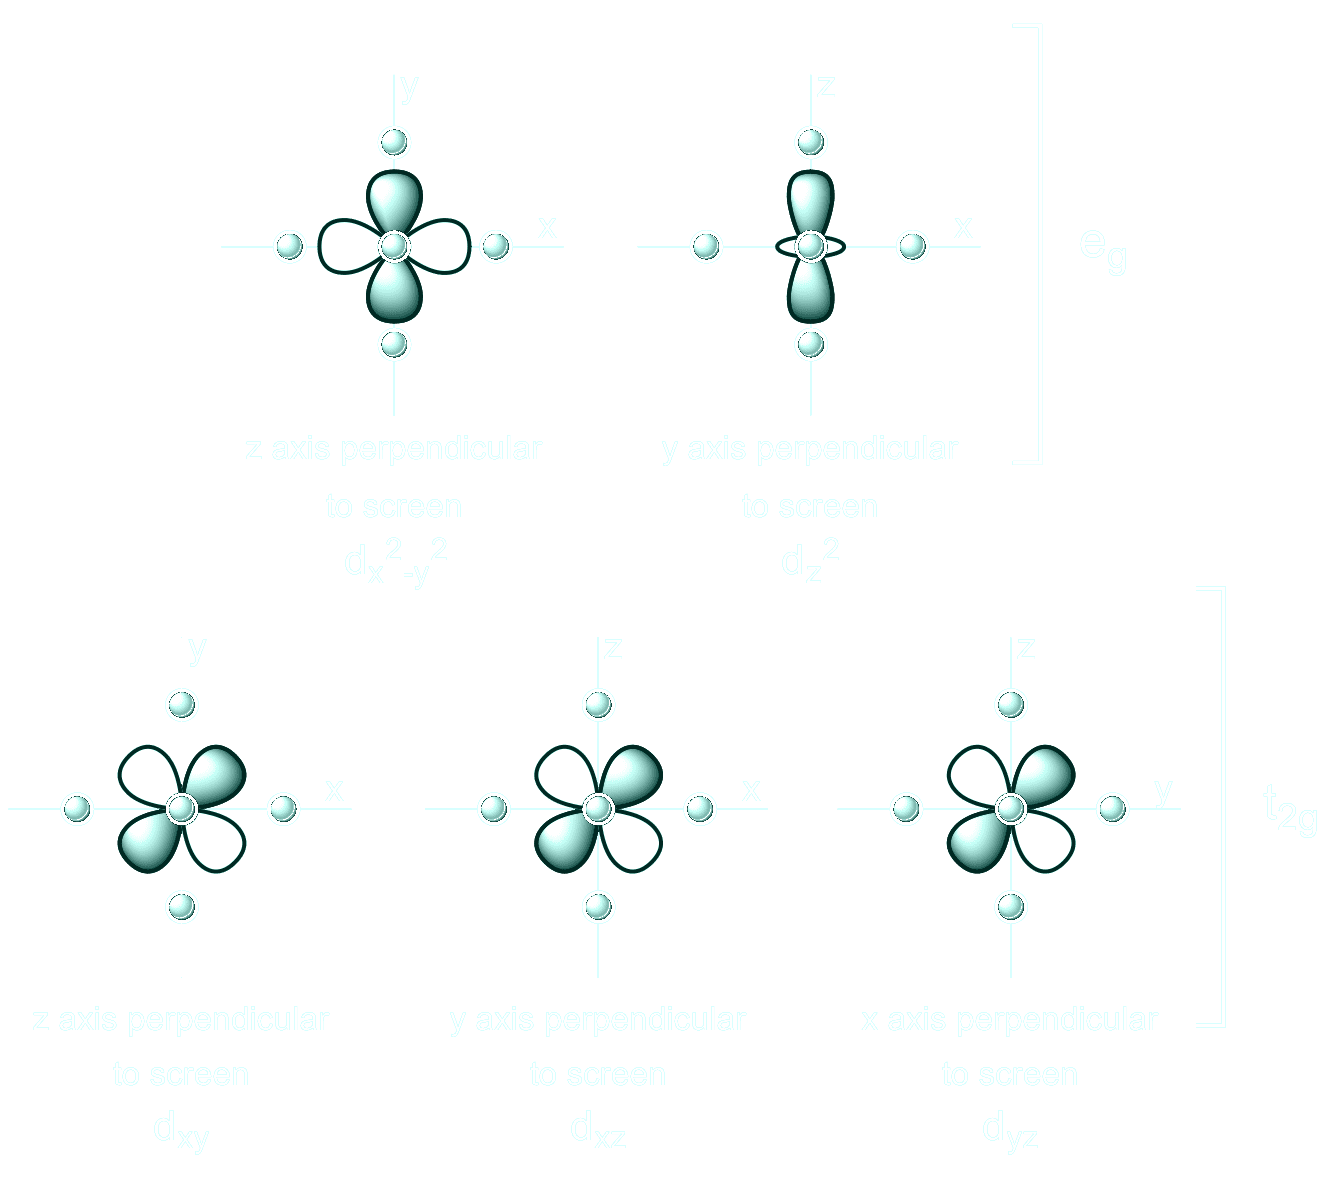
\includegraphics[width=.8\textwidth]
	{campo cristalino/octaedrico}

\resizebox{\textwidth}{!}{
\begin{modiagram}
	
	% left
	\AO(10mm){s}			{-0.10; }
	\AO(10mm){s}			{-0.05; }
	\AO[left](10mm){s}		{ 0.00; }
	\AO(10mm){s}			{ 0.05; }
	\AO(10mm){s}[label=d]	{ 0.10; }
	
	\node at (10.0mm, -1) 
	{\tiny 
		\begin{tabular}{c}
			Ausencia de 
		\\	campo exterior	
		\end{tabular}
	};
	
	% middle	
	\AO(40mm){s}			{0.90; }
	\AO(40mm){s}			{0.95; }
	\AO[middle](40mm){s}	{1.00; }
	\AO(40mm){s}			{1.05; }
	\AO(40mm){s}[label=d]	{1.10; }
	
	\node at (40mm,-1)
	{\tiny Campo Esférico};
	
	% right below
	\AO[right-below](70.0mm){s}[label=$yz$]{ .6; }
	\AO(77.5mm){s}[label=$xz$]{ .6; }
	\AO(85.0mm){s}[label=$xy$]{ .6; }
	
	% right above
	\AO[right-above]
	   (77.5mm){s}[label=$x^2$-$y^2$]	{1.6; }
	\AO(85.0mm){s}[label=$z^2$]		{1.6; }
	
	\node at (77.5mm, -1) 
	{\tiny Campo Octaédrico};
	
	\draw[<-|] 
	(65mm,1.6)
	-- node[above left]{\tiny $+0.6\,\Delta_{\text{oct}}$} 
	(65mm,1.0);
	
	\draw[->]
	(65mm,1.0)
	-- node[below left]{\tiny $-0.4\,\Delta_{\text{oct}}$}
	(65mm,0.6);
	
	\draw[<->] 
	(95mm,1.6) 
		node[left] {\tiny e\textsubscript{g}}
		node[below right]{\tiny $\Delta _{\text{oct}}$ }
	-- 
		node[above=2.5mm, right=4mm, rotate=-90]{\tiny=}
	(95mm,0.6) 
		node[left] {\tiny t\textsubscript{2g}}
		node[above right]{\tiny $10\,\text{Dq}$};
	
	\connect{
		left & middle, 
		middle & right-above, 
		middle & right-below
	}
	
	\EnergyAxis
	\node at (0,1)[above, rotate=90]{\tiny Energia};

\end{modiagram}
}



\end{tcolorbox}


% Tetraédrico
\subsection*{Complexo Tetaédrico}
\begin{tcolorbox}\centering

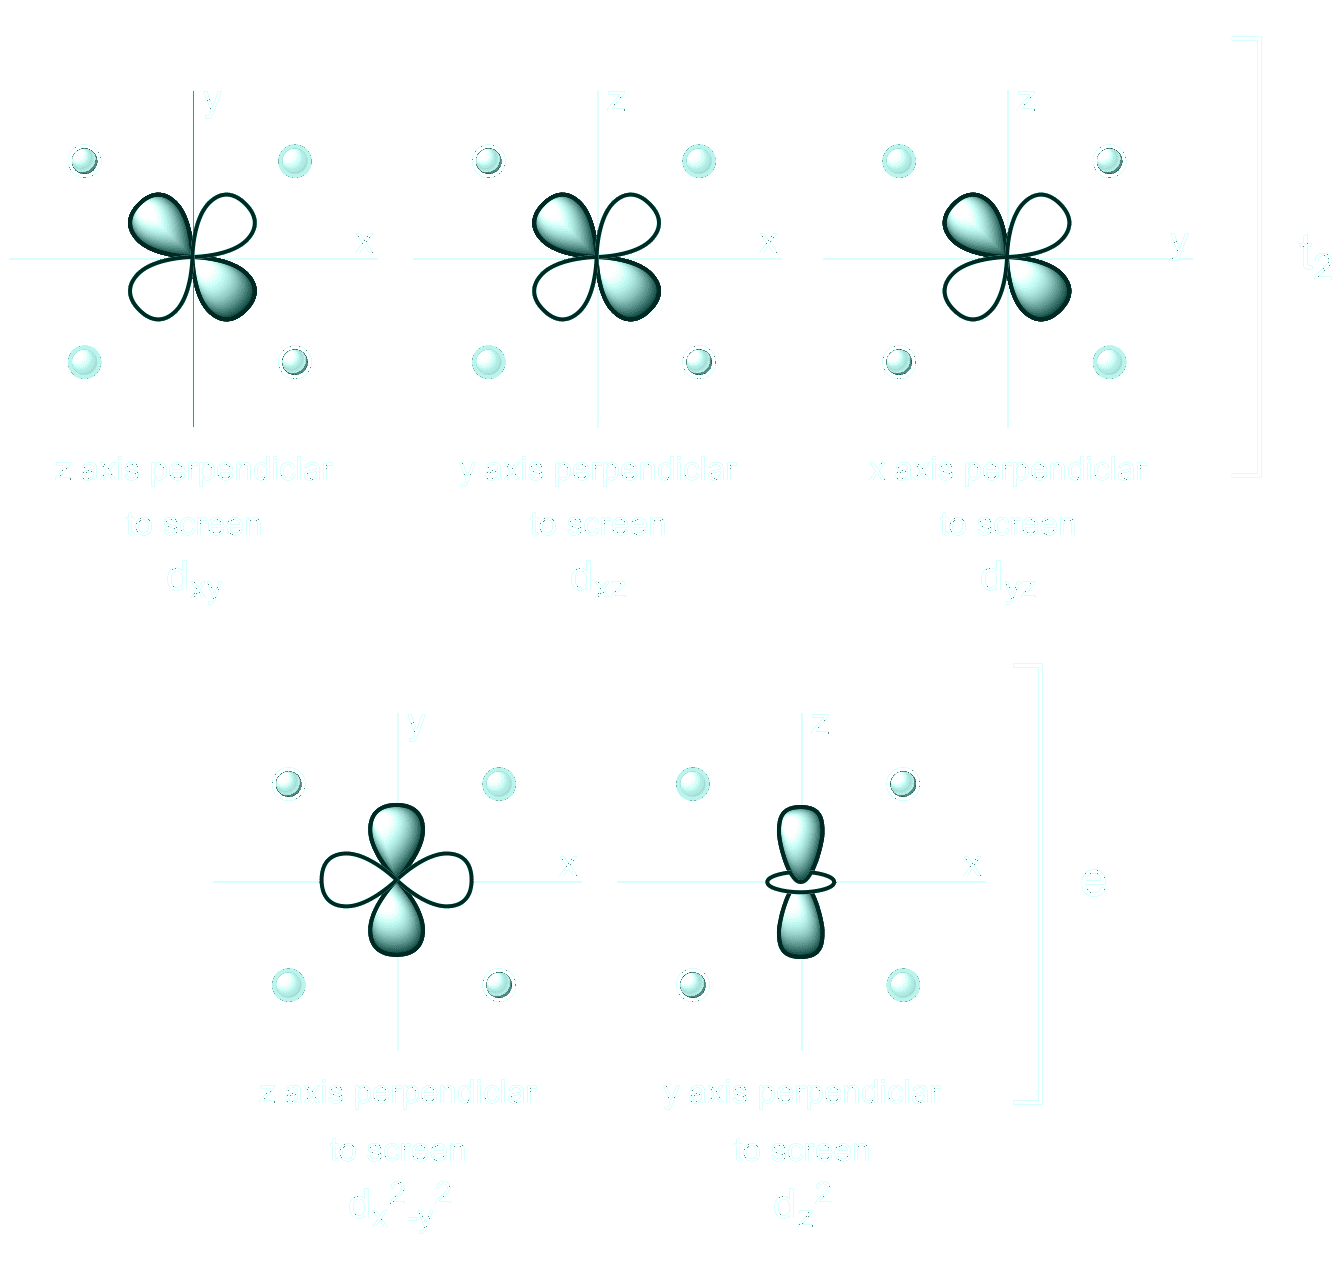
\includegraphics[width=.8\textwidth]
	{campo cristalino/tetraedrico}

\resizebox{\textwidth}{!}{
\begin{modiagram}
	
	% left
	\AO(10mm){s}			{-0.10; }
	\AO(10mm){s}			{-0.05; }
	\AO[left](10mm){s}		{ 0.00; }
	\AO(10mm){s}			{ 0.05; }
	\AO(10mm){s}[label=d]	{ 0.10; }
	
	\node at (10.0mm, -1) 
	{\tiny 
		\begin{tabular}{c}
			Ausencia de 
		\\	campo exterior	
		\end{tabular}
	};
	
	% middle	
	\AO(40mm){s}			{0.90; }
	\AO(40mm){s}			{0.95; }
	\AO[middle](40mm){s}	{1.00; }
	\AO(40mm){s}			{1.05; }
	\AO(40mm){s}[label=d]	{1.10; }
	
	\node at (40mm,-1)
	{\tiny Campo Esférico};
	
	% right above
	\AO[right-below]
	   	(70.0mm){s}[label=$yz$]{1.4; }
	\AO	(77.5mm){s}[label=$xz$]{1.4; }
	\AO	(85.0mm){s}[label=$xy$]{1.4; }
	
	% right below
	\AO[right-above]
	   (77.5mm){s}[label=$x^2$-$y^2$]	{0.4; }
	\AO(85.0mm){s}[label=$z^2$]		{0.4; }
	
	\node at (77.5mm, -1) 
	{\tiny Campo Tetraédrico};
	
	\draw[<-|] 
	(65mm,1.4)
	-- node[above left]{\tiny $+0.6\,\Delta_{\text{t}}$} 
	(65mm,1.0);
	
	\draw[->]
	(65mm,1.0)
	-- node[below left]{\tiny $-0.4\,\Delta_{\text{t}}$}
	(65mm,0.4);
	
	\draw[<->] 
	(95mm,1.4) 
		node[left] {\tiny t\textsubscript{2}}
		node[below right]{\tiny $\Delta _{\text{t}}$ }
	-- 
		node[above=2.5mm, right=3mm, rotate=-90]{\tiny=}
	(95mm,0.4) 
		node[left] {\tiny e}
		node[above right]{\tiny $10\,\text{Dq}$};
	
	\connect{
		left & middle, 
		middle & right-above, 
		middle & right-below
	}
	
	\EnergyAxis
	\node at (0,1)[above, rotate=90]{\tiny Energia};

\end{modiagram}
}

\end{tcolorbox}


\newpage


\begin{multicols}{2}

\subsection*{Campo fraco/Spin alto}
%\vspace{-5mm}

\begin{tcolorbox}\centering

\resizebox{!}{5cm}{
\begin{modiagram}
	
	% right below
	\AO[right-below]
		( 5.0mm){s}[label=$yz$]{-.4;pair}
	\AO	(12.5mm){s}[label=$xz$]{-.4;up}
	\AO	(20.0mm){s}[label=$xy$]{-.4;up}
	
	% right above
	\AO[right-above]
	   (12.5mm){s}[label=$x^2$-$y^2$]	{.6;up}
	\AO(20.0mm){s}[label=$z^2$]		{.6;up}
	
	\draw[<->] 
	(30mm,.6) node[left] {\tiny e\textsubscript{g}}
	-- node[right]
			{\tiny 
			\chemDelta\textsubscript{oct}
			$<$
			P
			}
	(30mm,-.4) node[left] {\tiny t\textsubscript{2g}};
	
	\draw[- Latex] (0,-2) -- (0,2.2);
	\node at (0,0)[above, rotate=90]{\tiny Energia};

\end{modiagram}
}

\end{tcolorbox}

%\vfill

\subsection*{Campo forte/Spin baixo}

\begin{tcolorbox}\centering

\resizebox{!}{5cm}{
\begin{modiagram}
	
	% right below
	\AO[right-below]
		( 5.0mm){s}[label=$yz$]{-1.2;pair}
	\AO	(12.5mm){s}[label=$xz$]{-1.2;pair}
	\AO	(20.0mm){s}[label=$xy$]{-1.2;pair}
	
	% right above
	\AO[right-above]
	   (12.5mm){s}[label=$x^2$-$y^2$]	{1.8;}
	\AO(20.0mm){s}[label=$z^2$]		{1.8;}
	
	\draw[<->] 
	(30mm, 1.8) node[left] {\tiny e\textsubscript{g}}
	-- node[right]
			{\tiny 
			\chemDelta\textsubscript{oct}
			$>$
			P
			}
	(30mm,-1.2) node[left] {\tiny t\textsubscript{2g}};
	
	\draw[- Latex] (0,-2) -- (0,2.2);
	\node at (0,0)[above, rotate=90]{\tiny Energia};
	
\end{modiagram}
}

\end{tcolorbox}

\end{multicols}


% talvez incluir em campo forte/fraco
\subsection{para/dia magnetismo}

\subsection{Fatores que influenciam}

%\begin{multicols}{2}
%\begin{enumerate}[left=0mm]
%	
%	\item Estado de oxidação do ion metálico
%	\item Natureza do ion  metálico
%	\item Natureza do Ligando
%	
%\end{enumerate}
%\end{multicols}

\subsubsection{Estado de Oxidação do ion metálico}

{


\setlength\tabcolsep{2mm}
%\renewcommand\arraystretch{1.25}

\newcommand\tsuchida[2]%
	{\cellcolor{Emph!#1!Black}%
		{\textcolor{White!#1!Emph!60!White}{\ch{#2}}}
	}

%for i in {0..8}                 
%do
%        echo "10.0+1.12*$i^2" | bc -l
%done

\subsubsection{Natureza do ion Metálico}
%
Diretamente proporconal:
\begin{itemize}
\item Estado de Oxidação
\item Periodo da tabela dos elementos
\end{itemize}
%

\begin{table}[H]\centering
\resizebox{\textwidth}{!}{
\begin{tabular}{ *{9}{c} }
	
	% 15 uniques
	
	\hline
	
%	\begin{tabular}{@{}*{13}{c}@{}}
	
	  \tsuchida{10.00}{				Mn^{2+}}
	& \tsuchida{11.12}{<\quad 		Ni^{2+}}
	& \tsuchida{14.48}{<\quad 		Co^{2+}}
	& \tsuchida{20.08}{<\quad 		Fe^{2+}}
	& \tsuchida{27.92}{<\quad 		V^{2+}}
	& \tsuchida{38.00}{<\quad 		Fe^{3+}}
	& \tsuchida{50.32}{<\quad 		Cr^{3+}}
	& \tsuchida{64.88}{<\quad 		V^{3+}}
	& \tsuchida{81.68}{<\quad 		Co^{3+}}
	
%	\end{tabular}
	
	\\ \hline

\end{tabular}
}
\caption{Série Espectroquímica ou Série de Tsuchida dos Metais}
\end{table}


\subsubsection{Natureza do Ligando}

\begin{table}[H]\centering
\resizebox{\textwidth}{!}{
\begin{tabular}{ *{13}{c} }
	
	% 15 uniques
	
	\hline
	
%	\begin{tabular}{@{}*{13}{c}@{}}
	
	  \tsuchida{10.000}{				I-}
	& \tsuchida{10.175}{<\quad 		Br-}
	& \tsuchida{10.700}{<\quad 		S^{2-}}
	& \tsuchida{11.575}{<\quad 		SCN-}
	& \tsuchida{11.900}{\lesssim\quad 	Cl-}
	& \tsuchida{12.800}{<\quad 		N3-}
	& \tsuchida{14.375}{<\quad 		F-}
	& \tsuchida{16.300}{<\quad 		NCO-}
	& \tsuchida{18.575}{<\quad 		OH-}
	& \tsuchida{21.200}{<\quad 		ox^{2-}}
	& \tsuchida{24.175}{<\quad 		H2O}
	& \tsuchida{27.500}{<\quad 		acac-}
	& \tsuchida{31.175}{<\quad 		NCS-}
	
%	\end{tabular}
	
	\\ \hline
	
%	\begin{tabular}{@{}*{13}{c}@{}}
	
	  \tsuchida{31.175}{				NCS-}
	& \tsuchida{35.200}{<\quad 		CH3CN}
	& \tsuchida{39.575}{<\quad 		gly}
	& \tsuchida{44.300}{<\quad 		py}
	& \tsuchida{49.375}{<\quad 		NH3}
	& \tsuchida{51.375}{\lesssim\quad 	en}
	& \tsuchida{54.800}{<\quad 		bpy}
	& \tsuchida{60.575}{<\quad 		phen}
	& \tsuchida{62.575}{\lesssim\quad 	NO2-}
	& \tsuchida{66.700}{<\quad	 	PPh3}
	& \tsuchida{66.700}{\approx\quad 	PR3}
	& \tsuchida{73.175}{<\quad 		CN-}
	& \tsuchida{77.000}{\lesssim\quad 	CO}
	
%	\end{tabular}
	
	\\ \hline

\end{tabular}
}
\caption{Série Espectroquímica ou Série de Tsuchida dos ligantes}
\end{table}
}

\subsection{Energia de Estabilização dos Campo de Ligandos EECL}

{\large\bfseries\boldmath
\begin{align*}
	\textbf{EECL}
=	(l*0.4-h*0.6)\,\chemDelta\textsubscript{oct}
-	n*\textbf{P}
\end{align*}
}

\begin{multicols}{2}
\begin{itemize}[left=0mm]
	
	\item $h$: Elétrons no campo de maior energia
	\item $l$: Elétrons no campo de menor energia
	\item $n$: Pares eletrônicos
	
\end{itemize}
\end{multicols}

\section*{Aplicações do Campo Cristalino}

\subsection{Espectro de Frequência de Absorção de Luz}



\end{document}
